\documentclass[table]{beamer}
%[]中可以使用draft、handout、screen、transparency、trancompress、compress等参数

%指定beamer的模式与主题
\mode<presentation>
{
  \usetheme{Madrid}
%\usetheme{Boadilla}
%\usecolortheme{default}
%\usecolortheme{orchid}
%\usecolortheme{whale}
%\usefonttheme{professionalfonts}
}

%\usetheme{Madrid}
%这里还可以选择别的主题:Bergen, Boadilla, Madrid, AnnArbor, CambridgeUS, Pittsburgh, Rochester, Warsaw, ...
%有导航栏的Antibes, JuanLesPins, Montpellier, ...
%有内容的Berkeley, PaloAlto, Goettingen, Marburg, Hannover, ...
%有最小导航栏的Berlin, Ilmenau, Dresden, Darmstadt, Frankfurt, Singapore, Szeged, ...
%有章和节表单的Copenhagen, Luebeck, Malmoe, Warsaw, ...

%\usecolortheme{default}
%设置内部颜色主题(这些主题一般改变block里的颜色);这个主题一般选择动物来命名
%这里还可以选择别的颜色主题,如默认的和有特别目的的颜色主题default,structure,sidebartab,全颜色主题albatross,beetle,crane,dove,fly,seagull,wolverine,beaver

%\usecolortheme{orchid}
%设置外部颜色主题(这些主题一般改变title里的颜色);这个主题一般选择植物来命名
%这里还可以选择别的颜色主题,如默认的和有特别目的的颜色主题lily,orchid,rose

%\usecolortheme{whale}
%设置字体主题;这个主题一般选择海洋动物来命名
%这里还可以选择别的颜色主题,如默认的和有特别目的的颜色主题whale,seahorse,dolphin

%\usefonttheme{professionalfonts}
%类似的还可以定义structurebold,structuresmallcapsserif,professionalfonts

% 控制 beamer 的风格,可以根据自己的爱好修改
%\usepackage{beamerthemesplit} %使用 split 风格
%\usepackage{beamerthemeshadow} %使用 shadow 风格
%\usepackage[width=2cm,dark,tab]{beamerthemesidebar}

%插入音标
%\usepackage{tipa}
%\AtBeginDocument{
  %\renewcommand\textipa{\fontencoding{T3}\selectfont}
%}
%\AtBeginDocument{
  %\renewcommand\textipa[2][r]{{\fontfamily{cm#1}\tipaencoding #2}}
%}
%\renewenvironment{IPA}[1][r]
 %{\fontfamily{cm#1}\tipaencoding}
 %{}

% 设定英文字体
%\usepackage{fontspec}
% Fix bugs for fontspec in TeXLive2015
\ifdefined\suppressfontnotfounderror
  \expandafter\let\csname xetex_suppressfontnotfounderror:D\endcsname
    \suppressfontnotfounderror
\else
  \expandafter\let\csname xetex_suppressfontnotfounderror:D\endcsname
    \luatexsuppressfontnotfounderror
\fi
\usepackage[no-math]{fontspec}
\setmainfont{Times New Roman}
\setsansfont{Arial}
\setmonofont{Courier New}

% 设定中文字体
\usepackage[BoldFont,SlantFont,CJKchecksingle,CJKnumber]{xeCJK}
%\setCJKmainfont[BoldFont={Adobe Heiti Std},ItalicFont={Adobe Kaiti Std}]{Adobe Song Std}
\setCJKmainfont[BoldFont={Adobe Heiti Std},ItalicFont={Adobe Kaiti Std}]{WenQuanYi Micro Hei}
\setCJKsansfont{Adobe Heiti Std}
\setCJKmonofont{Adobe Fangsong Std}
\punctstyle{hangmobanjiao}

\defaultfontfeatures{Mapping=tex-text}
\usepackage{xunicode}
\usepackage{xltxtra}

\XeTeXlinebreaklocale "zh"
\XeTeXlinebreakskip = 0pt plus 1pt minus 0.1pt

\usepackage{setspace}
\usepackage{colortbl,xcolor}
\usepackage{hyperref}
%\hypersetup{xetex,bookmarksnumbered=true,bookmarksopen=true,pdfborder=1,breaklinks,colorlinks,linkcolor=blue,filecolor=black,urlcolor=cyan,citecolor=green}
\hypersetup{xetex,bookmarksnumbered=true,bookmarksopen=true,pdfborder=1,breaklinks,colorlinks,linkcolor=cyan,filecolor=black,urlcolor=blue,citecolor=green}

% 插入图片
\usepackage{graphicx}
\graphicspath{{figures/}}
% 图文混排
%\usepackage{picins}
\usepackage{floatflt}

% 可能用到的包
\usepackage{amsmath,amssymb}
%插入多媒体
%\usepackage{media9}
%\usepackage{movie15}
\usepackage{multimedia}
\usepackage{multicol}
\usepackage{multirow}

% 定义一些自选的模板,包括背景、图标、导航条和页脚等,修改要慎重
% 设置背景渐变由10%的红变成10%的结构颜色
%\beamertemplateshadingbackground{red!10}{structure!10}
%\beamertemplatesolidbackgroundcolor{white!90!blue}
% 使所有隐藏的文本完全透明、动态,而且动态的范围很小
\beamertemplatetransparentcovereddynamic
% 使itemize环境中变成小球,这是一种视觉效果
\beamertemplateballitem
% 为所有已编号的部分设置一个章节目录,并且编号显示成小球
\beamertemplatenumberedballsectiontoc
% 将每一页的要素的要素名设成加粗字体
\beamertemplateboldpartpage

% item逐步显示时,使已经出现的item、正在显示的item、将要出现的item呈现不同颜色
\def\hilite<#1>{
 \temporal<#1>{\color{gray}}{\color{blue}}
    {\color{blue!25}}
}

\renewcommand{\today}{\number\year 年 \number\month 月 \number\day 日}

%五角星
\usepackage{MnSymbol}

%去除图表标题中的figure等
\usepackage{caption}
\captionsetup{labelformat=empty,labelsep=none}

\usepackage{tabu}
\usepackage{multirow}
%表格自动换行
\usepackage{tabularx} 

% 千分号
%\usepackage{textcomp}

%罗马数字
\makeatletter
\newcommand{\rmnum}[1]{\romannumeral #1}
\newcommand{\Rmnum}[1]{\expandafter\@slowromancap\romannumeral #1@}
\makeatother

%分栏
\usepackage{multicol}

%\usepackage{enumitem}
%\usepackage{enumerate}

%键盘
\usepackage{keystroke}

%插入源代码
\usepackage{listings}
\lstset{
  language=perl,                  % 程序语言名称:TeX, Perl, R, sh, bash, Awk
  basicstyle=\normalsize\tt,      %\tt指monospace字体族,程序源代码使用此族字体表示更加美观
  numbers=left,                   % 行号位置(左侧)
  numberstyle=\small,             % 行号字体的字号
  stepnumber=1,                   % 行号的显示步长
  numbersep=5pt,                  % 行号与代码间距
  backgroundcolor=\color{white},  % 背景色;需要 \usepackage{color}
  showspaces=false,               % 不显示空格
  showstringspaces=false,         % 不显示代码字符串中的空格标记
  showtabs=false,                 % 不显示 TAB
  tabsize=4, 
  frame=shadowbox,                % 把代码用带有阴影的框圈起来
  captionpos=b,                   % 标题位置
  breaklines=true,                % 对过长的代码自动断行
  breakatwhitespace=false,        % 断行只在空格处
  extendedchars=false,            % 解决代码跨页时,章节标题,页眉等汉字不显示的问题
  %escapeinside={\%*}{*},         % 跳脱字符,添加注释,暂时离开 listings 
  %escapeinside=``,
  commentstyle=\color{red!50!green!50!blue!50}\tt,  %浅灰色的注释
  rulesepcolor=\color{red!20!green!20!blue!20},     %代码块边框为淡青色
  keywordstyle=\color{blue!70}\bfseries\tt,         %代码关键字的颜色为蓝色,粗体
  identifierstyle=\tt,
  stringstyle=\tt,                % 代码字符串的特殊格式
  keepspaces=true,
  breakindent=1em,
  %breakindent=22pt,
  %breakindent=4em,
  breakautoindent=true,
  flexiblecolumns=true,
  aboveskip=1em,                  %代码块边框
  xleftmargin=2em,
  xrightmargin=2em
}

%\setbeamercolor{alerted text}{fg=magenta}
\setbeamercolor{bgcolor}{fg=yellow,bg=cyan}
%\setbeamercolor{itemize/enumerate body}{fg=green}

\begin{document}

%\includeonlyframes{current}

\logo{
\includegraphics[height=0.08\textwidth]{tijmu.png}}

% 在每个Section前都会加入的Frame
\AtBeginSection[]
{
  \begin{frame}<beamer>
    %\frametitle{Outline}
    \frametitle{教学提纲}
    \setcounter{tocdepth}{3}
    \begin{multicols}{2}
      \tableofcontents[currentsection,currentsubsection]
      %\tableofcontents[currentsection]
    \end{multicols}
  \end{frame}
}
% 在每个Subsection前都会加入的Frame
\AtBeginSubsection[]
{
  \begin{frame}<beamer>
%%\begin{frame}<handout:0>
%% handout:0 表示只在手稿中出现
    \frametitle{教学提纲}
    \setcounter{tocdepth}{3}
    \begin{multicols}{2}
    \tableofcontents[currentsection,currentsubsection]
    \end{multicols}
%% 显示在目录中加亮的当前章节
  \end{frame}
}

% 为当前幻灯片设置背景
%{
%\usebackgroundtemplate{
%\vbox to \paperheight{\vfil\hbox to
%\paperwidth{\hfil
\includegraphics[width=2in]{tijmu_charcoal.png}\hfil}\vfil}
%}
\begin{frame}[plain]
  \begin{center}
    {\Huge 分子生物计算\\}
    {\huge \textit{(Perl语言编程)}\\}
    \vspace{1cm}
    {\LARGE 天津医科大学\\}
    %\vspace{0.2cm}
    {\LARGE 生物医学工程与技术学院\\}
    \vspace{1cm}
    {\large 2016-2017学年上学期(秋)\\ 2014级生信班}
  \end{center}
\end{frame}
%}



%\includeonlyframes{current}

\title[Markdown]{第一章\quad Markdown标记语言}
\author[Yixf]{伊现富(Yi Xianfu)}
\institute[TIJMU]{天津医科大学(TIJMU)\\ 生物医学工程与技术学院}
\date{2016年11月}

\begin{frame}
  \titlepage
\end{frame}

\begin{frame}[plain,label=current]
  \frametitle{教学提纲}
  \setcounter{tocdepth}{3}
  \begin{multicols}{2}
    \tableofcontents
  \end{multicols}
\end{frame}


\section{Markdown简介}
\begin{frame}
  \frametitle{Markdown | 简介}
  Markdown 是一种轻量级标记语言,创始人为约翰·格鲁伯(John Gruber)。它允许人们“使用易读易写的纯文本格式编写文档,然后转换成有效的XHTML(或者HTML)文档”。这种语言吸收了很多在电子邮件中已有的纯文本标记的特性。
  \begin{figure}
    \centering
    
\includegraphics[width=7cm]{c1.markdown.logo.jpg}
  \end{figure}
\end{frame}

\begin{frame}
  \frametitle{Markdown | 宗旨}
  Markdown的目标是实现“易读易写”,成为一种适用于网络的\textit{书写}语言。\\
  \vspace{1em}
一份使用Markdown格式撰写的文件应该可以直接以纯文本发布,并且看起来不会像是由许多标签或是格式指令所构成。Markdown语法受到一些既有text-to-HTML格式的影响,包括Setext、atx、Textile、reStructuredText、Grutatext和EtText,而最大灵感来源其实是纯文本电子邮件的格式。\\
  \vspace{1em}
总之,Markdown的语法全由一些符号所组成,这些符号经过精挑细选,其作用一目了然。比如:在文字两旁加上星号,看起来就像\textbf{强调}。Markdown的列表看起来,嗯,就是列表。Markdown的区块引用看起来就真的像是引用一段文字,就像你曾在电子邮件中见过的那样。
\end{frame}

\begin{frame}
  \frametitle{Markdown | 兼容HTML}
Markdown的构想\textbf{不是}要使得HTML文档更容易书写。在我看来,HTML已经很容易写了。Markdown的理念是,能让文档更容易读、写和随意改。HTML是一种\textbf{发布}的格式,Markdown是一种\textbf{书写}的格式。因此,Markdown的格式语法只涵盖纯文本可以涵盖的范围。\\
  \vspace{1em}
不在Markdown涵盖范围之内的标签,都可以直接在文档里面用HTML撰写。不需要额外标注这是HTML或是Markdown;只要直接加标签就可以了。
\end{frame}

\begin{frame}
  \frametitle{Markdown | vs. HTML}
  \begin{figure}
    \centering
    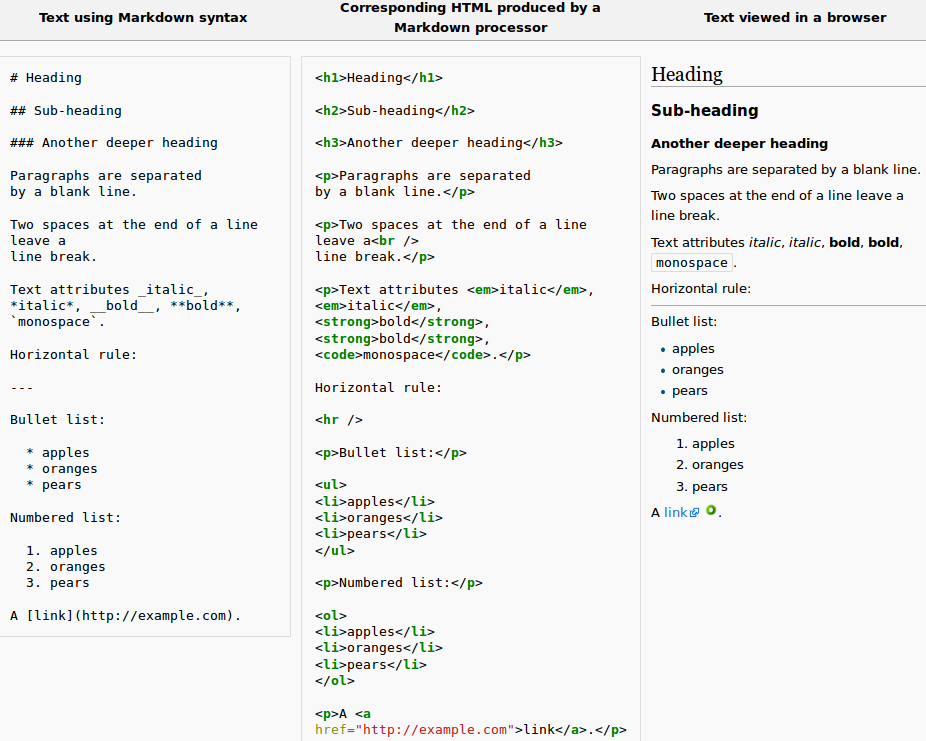
\includegraphics[width=0.8\textwidth]{c1.markdown.html.png}
  \end{figure}
\end{frame}

\begin{frame}
  \frametitle{Markdown | 用户}
  \begin{itemize}
    \item Bitbucket提供Markdown作为编写项目README文档的其中一种标记语言。
    \item GitHub使用Markdown的一个分支版本来格式化评论、消息以及其它内容。
    \item Reddit的编辑器使用了Markdown语法。
    \item Stack Overflow以及其他Stack Exchange Network网站使用一种Markdown的分支作为它的文章格式化系统。
    \item 图灵社区使用Markdown语法供用户写作电子书。
    \item 简书写作网站支持Markdown。
    \item 为知笔记是一种类似印象笔记的笔记软件,支持使用Markdown语法编辑笔记。
    \item ……
  \end{itemize}
\end{frame}

\begin{frame}
  \frametitle{Markdown | 编辑器}
作为一种小型标记语言,Markdown很容易阅读,也很容易用普通的文本编辑器编辑。另外也有一些编辑器专为Markdown设计,可以直接预览文档的样式。
  \begin{itemize}
    \item Cmd Markdown编辑阅读器:支持实时同步预览,区分写作和阅读模式,支持在线存储,分享文稿网址。
    \item Dillinger.io:一个在线Markdown编辑器,提供实时预览以及到GitHub和Dropbox的拓展链接。
    \item 简书:一个在线Markdown编辑器与阅读社区,支持实时预览,提供分享网址。
    \item Mou:一个Mac OS X上的Markdown编辑器。
    \item MarkdownPad:Windows上的全功能Markdown编辑器。
    \item PageDown:一个Javascript写的``WYSIWYM"(所见即所得)Markdown编辑器 (来自 StackOverflow)
    \item IPython Notebook:以IPython为后台,利用浏览器做IDE,支持Markdown与\LaTeX 公式。
    \item ……
  \end{itemize}
\end{frame}

\begin{frame}
  \frametitle{Markdown | 编辑器 | 免费}
  \begin{itemize}
    \item Windows平台
      \begin{itemize}
        \item MarkdownPad
	      \item MarkPad
      \end{itemize}
    \item Linux平台
      \begin{itemize}
        \item Typora
        \item Haroopad
        \item Remarkable
        \item ReText
        \item MdCharm
      \end{itemize}
    \item Mac平台:Mou
    \item 在线编辑器
      \begin{itemize}
	\item Markable.in
	\item Dillinger.io
      \end{itemize}
    \item 浏览器插件:MaDe (Chrome)
    \item 高级应用:Sublime Text 2 + MarkdownEditing
  \end{itemize}
\end{frame}

\begin{frame}
  \frametitle{Markdown | 编辑器 | Vim}
  \begin{block}{Vim插件管理器}
    \href{https://github.com/VundleVim/Vundle.vim}{Vundle}: the plug-in manager for Vim
  \end{block}
  \pause
  \begin{block}{Vim的Markdown插件}
    \begin{itemize}
      \item \href{https://github.com/plasticboy/vim-markdown}{vim-markdown}: Syntax highlighting, matching rules and mappings for the original Markdown and extensions.
      \item \href{https://github.com/suan/vim-instant-markdown}{vim-instant-markdown}: Instant Markdown previews from Vim! 
    \end{itemize}
  \end{block}
\end{frame}

\section{基本语法}
\subsection{区块元素}
\begin{frame}
  \frametitle{基本语法 | 区块元素 | 段落和换行}
一个Markdown段落是由一个或多个连续的文本行组成,它的\textcolor{red}{前后要有一个以上的空行}(空行的定义是显示上看起来像是空的,便会被视为空行。比方说,若某一行只包含空格和制表符,则该行也会被视为空行)。普通段落不该用空格或制表符来缩进。\\
  \vspace{1em}
“由一个或多个连续的文本行组成”这句话其实暗示了Markdown允许段落内的强迫换行(插入换行符),这个特性和其他大部分的text-to-HTML格式不一样。\\
  \vspace{1em}
在文本中输入的换行会从最终生成的结果中删除,浏览器会根据可用空间自动换行。如果想\textcolor{red}{强迫换行},可以在行尾插入至少两个空格。
\end{frame}

\begin{frame}[fragile]
  \frametitle{基本语法 | 区块元素 | 标题}
  Markdown支持两种标题的语法,类Setext和类atx形式。
  \begin{itemize}
    \item 类Setext形式是用底线的形式,利用 \verb|=|(最高阶标题)和 \verb|-|(第二阶标题)。任何数量的 \verb|=| 和 \verb|-| 都可以有效果。
    \item 类atx形式则是在行首插入1到6个 \verb|#|,对应到标题1到6阶。你可以选择性地“闭合”类atx样式的标题,这纯粹只是美观用的,若是觉得这样看起来比较舒适,你就可以在行尾加上 \verb|#|,而行尾的 \verb|#|数量也不用和开头一样(行首的井字符数量决定标题的阶数)。
  \end{itemize}
\end{frame}

\begin{frame}[fragile]
  \frametitle{基本语法 | 区块元素 | 标题 | 类Setext形式}
\begin{lstlisting}[language=]
This is an H1
=============

This is an H2
-------------
\end{lstlisting}
\pause
\begin{block}{预览}
{\LARGE This is an H1}\\
{\Large This is an H2}
\end{block}
\end{frame}

\begin{frame}[fragile]
  \frametitle{基本语法 | 区块元素 | 标题 | \alert{类atx形式}}
\begin{lstlisting}[language=]
# This is an H1
## This is an H2
### This is an H3
#### This is an H4
##### This is an H5
###### This is an H6
\end{lstlisting}
\pause
\begin{block}{预览}
{\LARGE This is an H1}\\
{\Large This is an H2}\\
{\large This is an H3}\\
{\normalsize This is an H4}\\
{\small This is an H5}\\
{\footnotesize This is an H6}
\end{block}
\end{frame}

\begin{frame}[fragile]
  \frametitle{基本语法 | 区块元素 | \alert{区块引用}}
  Markdown标记区块引用是使用类似email中用 \verb|>|的引用方式,看起来像是你自己先断好行,然后在每行的最前面加上 \verb|>|。\\
\begin{lstlisting}[language=]
>半亩方塘一鉴开,天光云影共徘徊。
>问渠那得清如许?为有源头活水来。
\end{lstlisting}
\end{frame}

\begin{frame}[fragile]
  \frametitle{基本语法 | 区块元素 | 区块引用}
  Markdown也允许你偷懒只在整个段落的第一行最前面加上 \verb|>|。\\
\begin{lstlisting}[language=]
>古之学者必有师。师者,所以传道受业解惑也。人非生而知之者,孰能无惑?惑而不从师,其为惑也,终不解矣。生乎吾前,其闻道也固先乎吾,吾从而师之;生乎吾後,其闻道也亦先乎吾,吾从而师之。吾师道也,夫庸知其年之先後生於吾乎!是故无贵无贱无长无少,道之所存,师之所存也。
>圣人无常师。孔子师郯子、苌子、师襄、老聃。郯子之徒,其贤不及孔子。孔子曰:“三人行,必有我师。”是故弟子不必不如师,师不必贤於弟子。闻道有先後,术业有专攻,如是而已。
\end{lstlisting}
\end{frame}

\begin{frame}[fragile]
  \frametitle{基本语法 | 区块元素 | 区块引用}
  区块引用可以嵌套(例如:引用内的引用),只要根据层次加上不同数量的 \verb|>|即可。\\
\begin{lstlisting}[language=]
>圣人无常师。孔子师郯子、苌子、师襄、老聃。郯子之徒,其贤不及孔子。孔子曰:
>
>>三人行,必有我师。
>
>是故弟子不必不如师,师不必贤於弟子。闻道有先後,术业有专攻,如是而已。
\end{lstlisting}
\end{frame}

\begin{frame}[fragile]
  \frametitle{基本语法 | 区块元素 | 区块引用}
  引用的区块内也可以使用其他的Markdown语法,包括标题、列表、代码区块等。
\begin{lstlisting}[language=]
>## 观书有感
>#### **朱熹**(*南宋*)
>半亩方塘一鉴开,天光云影共徘徊。
>问渠那得清如许?为有源头活水来。
\end{lstlisting}
\end{frame}

\begin{frame}[fragile]
  \frametitle{基本语法 | 区块元素 | \alert{列表}}
  \begin{block}{列表}
    Markdown支持无序列表和有序列表。\\
    \vspace{1em}
 列表项目标记通常是放在最左边,但是其实也可以缩进,最多3个空格,项目标记后面则一定要接着至少一个空格或制表符。
  \end{block}
  \pause
  \begin{block}{无序列表}
    无序列表使用星号(\verb|*|)、加号(\verb|+|)或是减号(\verb|-|)作为列表标记。
  \end{block}
  \pause
  \begin{block}{有序列表}
    有序列表则使用数字接着一个英文句点。(在列表标记上使用的数字并不会影响输出的HTML结果)
  \end{block}
\end{frame}

\begin{frame}[fragile]
  \frametitle{基本语法 | 区块元素 | 列表 | \alert{无序列表}}
  \begin{columns}
    \column{0.3\textwidth}
\begin{lstlisting}[language=]
* Red
* Green
* Blue
\end{lstlisting}
    \column{0.3\textwidth}
\begin{lstlisting}[language=]
+ Red
+ Green
+ Blue
\end{lstlisting}
    \column{0.3\textwidth}
\begin{lstlisting}[language=]
- Red
- Green
- Blue
\end{lstlisting}
  \end{columns}
  \begin{columns}
    \column{0.3\textwidth}
    \column{0.3\textwidth}
  \begin{block}{预览}
    \begin{itemize}
      \item Red
      \item Green
      \item Blue
    \end{itemize}
  \end{block}
    \column{0.3\textwidth}
  \end{columns}
\end{frame}

\begin{frame}[fragile]
  \frametitle{基本语法 | 区块元素 | 列表 | \alert{有序列表}}
  \begin{columns}
    \column{0.3\textwidth}
\begin{lstlisting}[language=]
1. Red
2. Green
3. Blue
\end{lstlisting}
    \column{0.3\textwidth}
\begin{lstlisting}[language=]
1. Red
1. Green
1. Blue
\end{lstlisting}
    \column{0.3\textwidth}
\begin{lstlisting}[language=]
3. Red
1. Green
5. Blue
\end{lstlisting}
  \end{columns}
  \begin{columns}
    \column{0.3\textwidth}
    \column{0.3\textwidth}
  \begin{block}{预览}
    \begin{enumerate}
      \item Red
      \item Green
      \item Blue
    \end{enumerate}
  \end{block}
    \column{0.3\textwidth}
  \end{columns}
\end{frame}

\begin{frame}[fragile]
  \frametitle{基本语法 | 区块元素 | 列表 | 多个段落}
  列表项目可以包含多个段落,每个项目下的段落都必须缩进4个空格或是1个制表符。
\begin{lstlisting}[language=]
1.  This is a list item with two paragraphs.

    This is the second paragraph.

2.  This is another...
\end{lstlisting}
\pause
\begin{lstlisting}[language=]
1.  This is a list item with two paragraphs.

This is the second paragraph.

2.  This is another...
\end{lstlisting}
\end{frame}

\begin{frame}[fragile]
  \frametitle{基本语法 | 区块元素 | 列表 | 引用}
  如果要在列表项目内放进引用,那么 \verb|>|就需要缩进:
\begin{lstlisting}[language=]
*   A list item with a blockquote:

    > This is a blockquote
    > inside a list item.
\end{lstlisting}
\end{frame}

\begin{frame}[fragile]
  \frametitle{基本语法 | 区块元素 | 列表 | 代码区块}
  如果要在列表中放代码区块的话,该区块就需要缩进两次,也就是8个空格或是2个制表符:
\begin{lstlisting}[language=]
*   A list item with a code block:

        #!/usr/bin/perl
        print "Hello, world!\n";
\end{lstlisting}
\end{frame}

\begin{frame}[fragile]
  \frametitle{基本语法 | 区块元素 | 列表 | 避免}
  项目列表很可能会不小心产生,也就是在行首出现数字-句点-空白的时候:
\begin{lstlisting}[language=]
1986. What a great season.
\end{lstlisting}
\pause
  要避免这样的状况,可以在句点前面加上反斜线:
\begin{lstlisting}[language=]
1986\. What a great season.
\end{lstlisting}
\end{frame}

\begin{frame}[fragile]
  \frametitle{基本语法 | 区块元素 | \alert{代码区块}}
和程序相关的写作或是标签语言源代码通常会有已经排版好的代码区块,对于这些区块,通常我们并不希望它以一般段落文件的方式去排版,而是照原来的样子显示。\\
  \vspace{1em}
  要在Markdown中建立代码区块很简单,只要简单地缩进4个空格或是1个制表符就可以:
\begin{lstlisting}[language=]
A normal paragraph followed by a Perl script:

    #!/usr/bin/perl
    print "Hello, world!\n";
\end{lstlisting}
\end{frame}

\begin{frame}[fragile]
  \frametitle{基本语法 | 区块元素 | 代码区块}
  \begin{itemize}
    \item 每行一阶的缩进,即4个空格或是1个制表符,都会被移除。
    \item 一个代码区块会一直持续到没有缩进的那一行(或是文件结尾)。
    \item 在代码区块里面,\verb|&|、\verb|<|和 \verb|>|会自动转成HTML实体,这样的方式让你非常容易使用Markdown插入范例用的HTML源代码——只需要复制贴上,再加上缩进就可以了——剩下的Markdown都会帮你处理。
    \item 代码区块中,一般的Markdown语法不会被转换,像是星号便只是星号,这表示你可以很容易地以Markdown语法撰写Markdown语法相关的文件。
  \end{itemize}
\end{frame}

\begin{frame}[fragile]
  \frametitle{基本语法 | 区块元素 | 引用 vs. 代码}
\begin{lstlisting}[language=]
>May the Force be with you!
\end{lstlisting}
  \pause
\begin{lstlisting}[language=]
    #!/usr/bin/perl
    print "Hello, world!\n";
\end{lstlisting}
\end{frame}

\begin{frame}[fragile]
  \frametitle{基本语法 | 区块元素 | \alert{分割线}}
    你可以在一行中用三个以上的星号、减号、下划线来建立一个分隔线,行内不能有其他东西。你也可以在星号、减号或者下划线中间插入空格。
\begin{lstlisting}[language=]
* * *

***

*****

- - -

---------------------------------------

___

_ _ _ _ _
\end{lstlisting}
\end{frame}

\subsection{区段元素}
\begin{frame}[fragile]
  \frametitle{基本语法 | 区段元素 | 链接}
  Markdown 支持两种形式的链接语法: 行内式和参考式两种形式。\\
  \vspace{1em}
  不管是哪一种,链接文字都是用\verb|[ ]|(方括号)来标记。
\end{frame}

\begin{frame}[fragile]
  \frametitle{基本语法 | 区段元素 | 链接 | \alert{行内式}}
  要建立一个行内式的链接,只要在方块括号后面紧接着圆括号并插入网址链接即可,如果你还想要加上链接的title文字,只要在网址后面,用双引号把title文字包起来即可:
\begin{lstlisting}[language=]
This is [an example](http://example.com/ "Title") inline link.

[This link](http://example.net/) has no title attribute.
\end{lstlisting}
\pause
如果你是要链接到同样主机的资源,可以使用相对路径:
\begin{lstlisting}[language=]
See my [About](/about/) page for details.
\end{lstlisting}
\end{frame}

\begin{frame}[fragile]
  \frametitle{基本语法 | 区段元素 | 链接 | \alert{参考式}}
  参考式的链接是在链接文字的括号后面再接上另一个方括号,而在第二个方括号里面要填入用以辨识链接的标记。你也可以选择性地在两个方括号中间加上一个空格。
\begin{lstlisting}[language=]
This is [an example][id] reference-style link.

This is [an example] [id] reference-style link.
\end{lstlisting}
接着,在文件的任意处,你可以把这个标记的链接内容定义出来:
\begin{lstlisting}[language=]
[id]: http://example.com/  "Optional Title Here"
\end{lstlisting}
\pause
网址定义只有在产生链接的时候用到,并不会直接出现在文件之中。
\end{frame}

\begin{frame}[fragile]
  \frametitle{基本语法 | 区段元素 | 链接 | 参考式 | \alert{定义形式}}
  \begin{itemize}
    \item 方括号(前面可以选择性地加上至多三个空格来缩进),里面输入链接文字
    \item 接着一个冒号
    \item 接着一个以上的空格或制表符
    \item 接着链接的网址
    \item 选择性地接着title内容,可以用单引号、双引号或是小括号包着
  \end{itemize}
\begin{lstlisting}[language=]
[foo]: http://example.com/  "Optional Title Here"
[foo]: http://example.com/  'Optional Title Here'
[foo]: http://example.com/  (Optional Title Here)
\end{lstlisting}
\end{frame}

\begin{frame}[fragile]
  \frametitle{基本语法 | 区段元素 | 链接 | 参考式 | 补充}
  链接网址也可以用尖括号包起来:
\begin{lstlisting}[language=]
[id]: <http://example.com/>  "Optional Title Here"
\end{lstlisting}
\pause
也可以把title属性放到下一行,也可以加一些缩进,若网址太长的话,这样会比较好看:
\begin{lstlisting}[language=]
[id]: http://example.com/longish/path/to/resource/here
    "Optional Title Here"
\end{lstlisting}
\pause
链接辨别标签可以有字母、数字、空白和标点符号,但是并不区分大小写,因此下面两个链接是一样的:
\begin{lstlisting}[language=]
[link text][a]
[link text][A]
\end{lstlisting}
\end{frame}

\begin{frame}[fragile]
  \frametitle{基本语法 | 区段元素 | 链接 | 参考式 | 隐式}
隐式链接标记功能让你可以省略指定链接标记,这种情形下,链接标记会视为等同于链接文字。要用隐式链接标记只要在链接文字后面加上一个空的方括号。比如要让“Google”链接到google.com:
\begin{lstlisting}[language=]
[Google][]
\end{lstlisting}
然后定义链接内容:
\begin{lstlisting}[language=]
[Google]: http://google.com/
\end{lstlisting}
\pause
由于链接文字可能包含空白,所以这种简化型的标记内也许包含多个单词:
\begin{lstlisting}[language=]
Visit [Daring Fireball][].
\end{lstlisting}
然后接着定义链接:
\begin{lstlisting}[language=]
[Daring Fireball]: http://daringfireball.net/
\end{lstlisting}
\end{frame}

\begin{frame}
  \frametitle{基本语法 | 区段元素 | 链接 | 参考式 | 补充}
链接的定义可以放在文件中的任何一个地方,我比较偏好直接放在链接出现段落的后面,你也可以把它放在文件最后面,就像是注解一样。\\
  \vspace{1em}
参考式的链接其实重点不在于它比较好写,而是它比较好读。使用Markdown的参考式链接,可以让文件更像是浏览器最后产生的结果。通过把一些标记相关的元数据移到段落文字之外,就可以增加链接而不让文章的阅读感觉被打断。
\end{frame}

\begin{frame}[fragile]
  \frametitle{基本语法 | 区段元素 | 链接 | 范例 | 行内式 vs. 参考式}
\begin{lstlisting}[language=]
I get 10 times more traffic from [Google](http://google.com/ "Google") than from [Yahoo](http://search.yahoo.com/ "Yahoo Search") or [MSN](http://search.msn.com/ "MSN Search").
\end{lstlisting}
\pause
\begin{lstlisting}[language=]
I get 10 times more traffic from [Google] [1] than from [Yahoo] [2] or [MSN] [3].

  [1]: http://google.com/        "Google"
  [2]: http://search.yahoo.com/  "Yahoo Search"
  [3]: http://search.msn.com/    "MSN Search"
\end{lstlisting}
\end{frame}

\begin{frame}[fragile]
  \frametitle{基本语法 | 区段元素 | 链接 | 范例 | 显式 vs. 隐式}
\begin{lstlisting}[language=]
I get 10 times more traffic from [Google] [1] than from [Yahoo] [2] or [MSN] [3].

  [1]: http://google.com/       "Google"
  [2]: http://search.yahoo.com/ "Yahoo Search"
  [3]: http://search.msn.com/   "MSN Search"
\end{lstlisting}
\pause
\begin{lstlisting}[language=]
I get 10 times more traffic from [Google][] than from [Yahoo][] or [MSN][].

  [google]: http://google.com/       "Google"
  [yahoo]:  http://search.yahoo.com/ "Yahoo Search"
  [msn]:    http://search.msn.com/   "MSN Search"
\end{lstlisting}
\end{frame}

\begin{frame}[fragile]
  \frametitle{基本语法 | 区段元素 | \alert{强调}}
  Markdown使用星号(\verb|*|)和下划线(\verb|_|)作为标记强调字词的符号。分为强调(斜体)、加重强调(粗体)和特别强调(粗斜体)。
\begin{columns}
  \column{0.6\textwidth}
\begin{lstlisting}[language=]
*single asterisks*

_single underscores_

**double asterisks**

__double underscores__

***three asterisks***

___three underscores___
\end{lstlisting}
  \column{0.4\textwidth}
  \begin{block}{预览}
    \textit{single asterisks}\\
    \textit{single underscores}\\
    \textbf{double asterisks}\\
    \textbf{double underscores}\\
    \textbf{\textit{three asterisks}}\\
    \textbf{\textit{three underscores}}
  \end{block}
\end{columns}
\pause
你可以随便用你喜欢的样式,唯一的限制是,你用什么符号开启标签,就要用什么符号结束。
\end{frame}

\begin{frame}[fragile]
  \frametitle{基本语法 | 区段元素 | 强调}
  强调也可以直接插在文字中间:
\begin{lstlisting}[language=]
un*frigging*believable
\end{lstlisting}
\pause
  但是如果你的\verb|*|和\verb|_|两边都有空白的话,它们就只会被当成普通的符号。\\
  \vspace{1em}
\pause
  如果要在文字前后直接插入普通的星号或下划线,你可以用反斜线:
\begin{lstlisting}[language=]
\*this text is surrounded by literal asterisks\*
\end{lstlisting}
\end{frame}

\begin{frame}[fragile]
  \frametitle{基本语法 | 区段元素 | \alert{行内代码}}
  如果要标记一小段行内代码,你可以用反引号把它包起来(\verb|`|):
\begin{lstlisting}[language=]
Use the `printf()` function.
\end{lstlisting}
\pause
如果要在代码区段内插入反引号,你可以用多个反引号来开启和结束代码区段:
\begin{lstlisting}[language=]
``There is a literal backtick (`) here.``
\end{lstlisting}
\pause
代码区段的起始和结束端都可以放入一个空白,起始端后面一个,结束端前面一个,这样你就可以在区段的一开始就插入反引号:
\begin{lstlisting}[language=]
A single backtick in a code span: `` ` ``
  
A backtick-delimited string in a code span: `` `foo` ``
\end{lstlisting}
\end{frame}

\begin{frame}[fragile]
  \frametitle{基本语法 | 区段元素 | 图片}
  Markdown使用一种和链接很相似的语法来标记图片,同样也允许两种样式:行内式和参考式。\\
  \vspace{1em}
  到目前为止,Markdown还没有办法指定图片的宽高,如果你需要的话,你可以使用普通的 \verb|<img>|标签。
\end{frame}

\begin{frame}[fragile]
  \frametitle{基本语法 | 区段元素 | 图片 | \alert{行内式}}
  行内式的图片语法:
  \begin{itemize}
    \item 一个感叹号(!)
    \item 接着一个方括号,里面放上图片的替代文字
    \item 接着一个普通括号,里面放上图片的网址,最后还可以用引号包住并加上选择性的“title”文字。
  \end{itemize}
\begin{lstlisting}[language=]
![Alt text](/path/to/img.jpg)

![Alt text](/path/to/img.jpg "Optional title")
\end{lstlisting}
\end{frame}

\begin{frame}[fragile]
  \frametitle{基本语法 | 区段元素 | 图片 | \alert{参考式}}
\begin{lstlisting}[language=]
![Alt text][id]
\end{lstlisting}
“id”是图片参考的名称,图片参考的定义方式和链接参考一样:
\begin{lstlisting}[language=]
[id]: url/to/image  "Optional title attribute"
\end{lstlisting}
\end{frame}

\subsection{其他}
\begin{frame}[fragile]
  \frametitle{基本语法 | 其他 | \alert{自动链接}}
  Markdown支持以比较简短的自动链接形式来处理网址和电子邮件信箱,只要是用尖括号包起来,Markdown就会自动把它转成链接。一般网址的链接文字就和链接地址一样:
\begin{lstlisting}[language=]
<http://example.com/>
\end{lstlisting}
\pause
电子邮箱地址的自动链接也很类似,只是Markdown会先做一个编码转换的过程,把文字字符转成16进位码的HTML实体,这样的格式可以糊弄一些不好的邮址收集机器人:
\begin{lstlisting}[language=]
<address@example.com>
\end{lstlisting}
(这种作法虽然可以糊弄不少的机器人,但并不能全部挡下来,不过总比什么都不做好些。不管怎样,公开你的信箱终究会引来广告信件的。)
\end{frame}

\begin{frame}[fragile]
  \frametitle{基本语法 | 其他 | \alert{反斜线}}
Markdown可以利用反斜线来插入一些在语法中有其它意义的符号,支持以下这些符号前面加上反斜线来帮助插入普通的符号:
\begin{lstlisting}[language=]
\   反斜线
`   反引号
*   星号
_   下划线
{}  大括号
[]  中括号
()  小括号
#   井字号
+   加号
-   减号
.   英文句点
!   感叹号
\end{lstlisting}
\end{frame}

\begin{frame}[fragile]
  \frametitle{基本语法 | 其他 | \alert{脚注}}
使用这样的占位符号可以将脚注添加到文本中:\verb|[^1]|。另外,你可以使用“n”而不是数字的\verb|[^n]|。所以你可以不必担心使用哪个号码。在您的文章的结尾,你可以如下所示定义匹配的注脚,URL将变成链接:
\begin{lstlisting}[language=]
[^1]: This is my first footnote
[^n]: Visit http://ghost.org
[^n]: A final footnote
\end{lstlisting}
\begin{lstlisting}[language=]
Footnotes[^1] have a label[^label] and a definition[^!DEF].

[^1]: This is a footnote
[^label]: A footnote on "label"
[^!DEF]: The definition of a footnote.
\end{lstlisting}
\end{frame}

\begin{frame}[fragile]
  \frametitle{基本语法 | 其他 | 字体颜色}
  使用HTML语法来设定字体的颜色:
\begin{lstlisting}[language=HTML]
<font color="red">我是红色字体</font> 

<font color="green">我是绿色字体</font> 

<font color="blue">我是蓝色字体</font> 

<font color="#FF0000">我是红色字体</font> 

<font color="#00FF00">我是绿色字体</font> 

<font color="#0000FF">我是蓝色字体</font> 
\end{lstlisting}
\end{frame}

\section{扩展语法}
\begin{frame}[fragile]
  \frametitle{扩展语法 | 杂项}
\begin{lstlisting}[language=]
# 目录
[toc]

# 元数据
---
title: 小书匠语法使用手册
tags: 小书匠,语法,MARKDOWN,帮助
--- 

# 扩展的文字格式
~~添加删除线~~
++插入的文字++
==被记号的文字==
上角文字: 19^th^
下角文字: H~2~o
\end{lstlisting}
\end{frame}

\begin{frame}[fragile]
  \frametitle{扩展语法 | 杂项}
\begin{lstlisting}[language=]
# 印刷字替换
(c) (C) (r) (R) (tm) (TM) (p) (P) +-

# 缩写定义
The HTML specification is maintained by the W3C.
*[HTML]: Hyper Text Markup Language
*[W3C]:  World Wide Web Consortium
\end{lstlisting}
\end{frame}

\begin{frame}[fragile]
  \frametitle{扩展语法 | 杂项}
\begin{lstlisting}[language=]
# 待办事项
[ ] 未完成事项
[-] 未完成事项
[x] 完成事项
[X] 完成事项

# 定义
苹果
: 一种水果
: 一种品牌,计算机,手持设备
桔子
: 一种水果
\end{lstlisting}
\end{frame}

\begin{frame}[fragile]
  \frametitle{扩展语法 | \alert{代码}}
  标准Markdown基于缩进代码行或者4个空格位:
\begin{lstlisting}[language=]
    #!/usr/bin/perl
    print "Hello, world!\n";
\end{lstlisting}
  GFM(GitHub Flavored Markdown)使用三个反引号\verb|```|:
\begin{lstlisting}[language=]
```perl
#!/usr/bin/perl
print "Hello, world!\n";
```
\end{lstlisting}
\end{frame}

\begin{frame}[fragile]
  \frametitle{扩展语法 | \alert{表格}}
\begin{lstlisting}[language=]
Left align | Right align | Center align 
:-----------|------------:|:------------:
 This       |        This |     This     
 column     |      column |    column    
 will       |        will |     will     
 be         |          be |      be      
 left       |       right |    center    
 aligned    |     aligned |   aligned 

* Outer pipes on tables are optional
* Colon used for alignment (right versus left)
\end{lstlisting}
\end{frame}

\begin{frame}[fragile]
  \frametitle{扩展语法 | 公式}
\begin{lstlisting}[language=]
基于LaTeX公式语法,可以创建行内公式,例如 $\Gamma(n) = (n-1)!\quad\forall n\in\mathbb N$。或者块级公式:

$$E=mc^2$$

$$ x = \dfrac{-b \pm \sqrt{b^2 - 4ac}}{2a} $$

$$
\Gamma(z) = \int_0^\infty t^{z-1}e^{-t}dt\,.
$$
\end{lstlisting}
\end{frame}

\begin{frame}[fragile]
  \frametitle{扩展语法 | 流程图}
\begin{lstlisting}[language=]
```flow
st=>start: Start
op=>operation: Your Operation
cond=>condition: Yes or No?
e=>end

st->op->cond
cond(yes)->e
cond(no)->op
```
\end{lstlisting}
\end{frame}

\begin{frame}[fragile]
  \frametitle{扩展语法 | 序列图/时序图}
\begin{lstlisting}[language=]
```seq
Alice->Bob: Hello Bob, how are you?
Note right of Bob: Bob thinks
Bob-->Alice: I am good thanks!
```
\end{lstlisting}
\end{frame}

\section{语法参考卡片}
\begin{frame}
  \frametitle{语法参考卡片}
  \begin{figure}
    \centering
    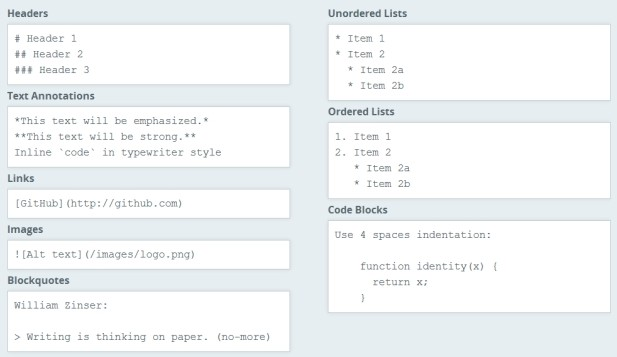
\includegraphics[width=12cm]{c1.markdown.cheatsheet.01.png}
  \end{figure}
\end{frame}

\begin{frame}
  \frametitle{语法参考卡片}
  \begin{figure}
    \centering
    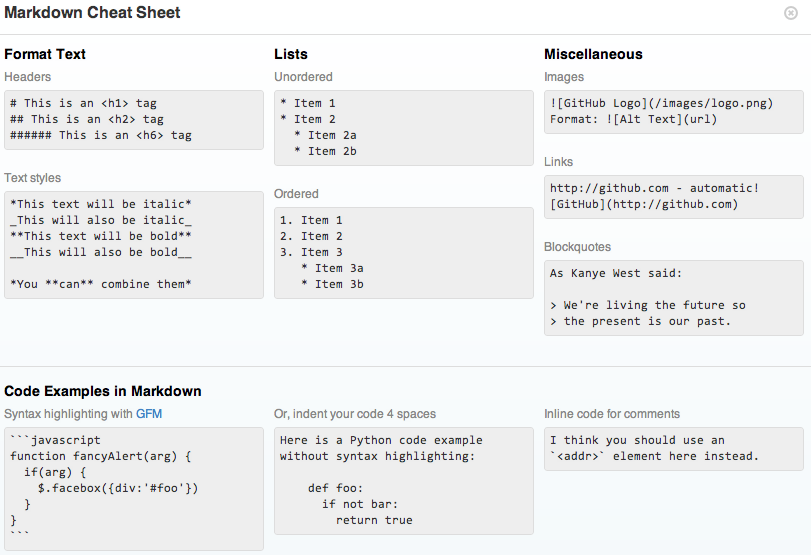
\includegraphics[width=11cm]{c1.markdown.cheatsheet.02.png}
  \end{figure}
\end{frame}

\begin{frame}
  \frametitle{语法参考卡片}
  \begin{figure}
    \centering
    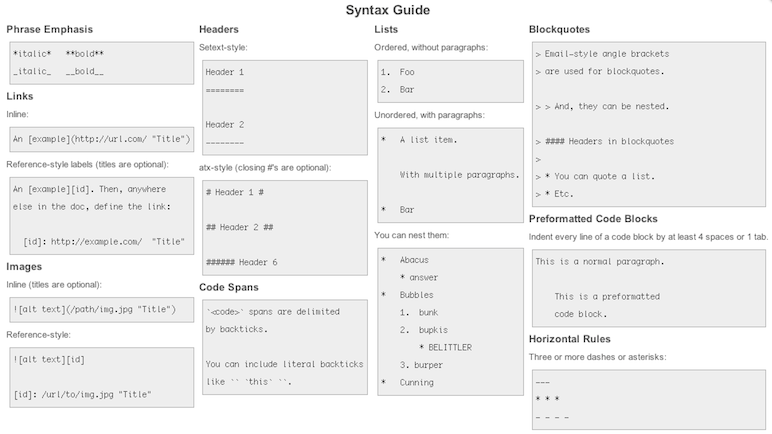
\includegraphics[width=12cm]{c1.markdown.cheatsheet.03.png}
  \end{figure}
\end{frame}

\begin{frame}
  \frametitle{语法参考卡片}
  \begin{figure}
    \centering
    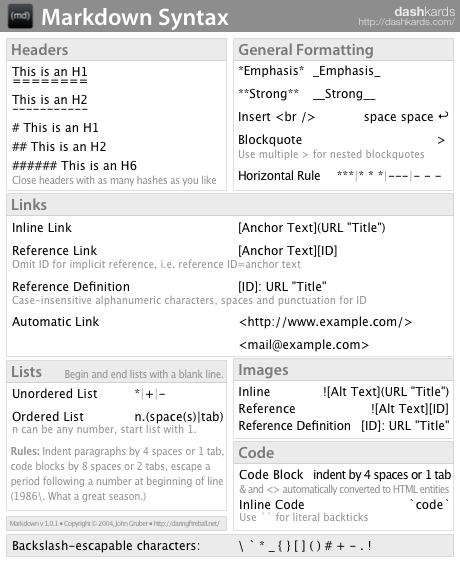
\includegraphics[width=9cm,height=8cm]{c1.markdown.cheatsheet.04.png}
  \end{figure}
\end{frame}

\begin{frame}
  \frametitle{语法参考卡片}
  \begin{figure}
    \centering
    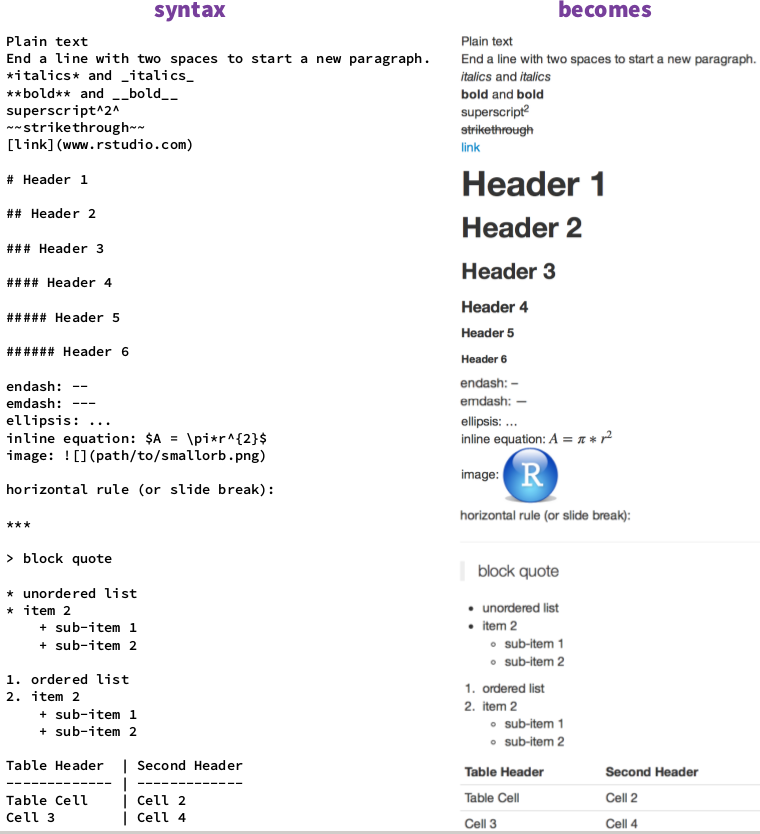
\includegraphics[width=9cm,height=8cm]{c1.markdown.cheatsheet.05.png}
  \end{figure}
\end{frame}

\section{可重复性研究}
\begin{frame}
  \frametitle{可重复性研究}
  \begin{block}{可重复性研究(Reproducible Research)}
    \begin{itemize}
      \item 代码、数据、结果集成在一起。
      \item RStudio (R + Markdown + knitr)
    \end{itemize}
  \end{block}
  \pause
  \begin{block}{参考链接}
    \begin{itemize}
      \item \href{https://github.com/yihui/r-ninja/blob/master/11-auto-report.md}{自动化报告}
      \item \href{http://cos.name/2012/06/reproducible-research-with-knitr/}{knitr与可重复的统计研究(花絮篇)}
    \end{itemize}
  \end{block}
\end{frame}

\section{格式转换}
\begin{frame}
  \frametitle{格式转换 | pandoc | 简介}
  pandoc是由John MacFarlane开发的标记语言转换工具,可实现不同标记语言间的格式转换,堪称该领域中的“瑞士军刀”。\\
  \vspace{1em}
  pandoc使用Haskell语言编写,以命令行形式实现与用户的交互,可支持多种操作系统。\\
  \vspace{1em}
  pandoc采用GNU GPL授权协议发布,属于自由软件。
\end{frame}

\begin{frame}
  \frametitle{格式转换 | pandoc | 支持格式}
  \begin{figure}
    \centering
    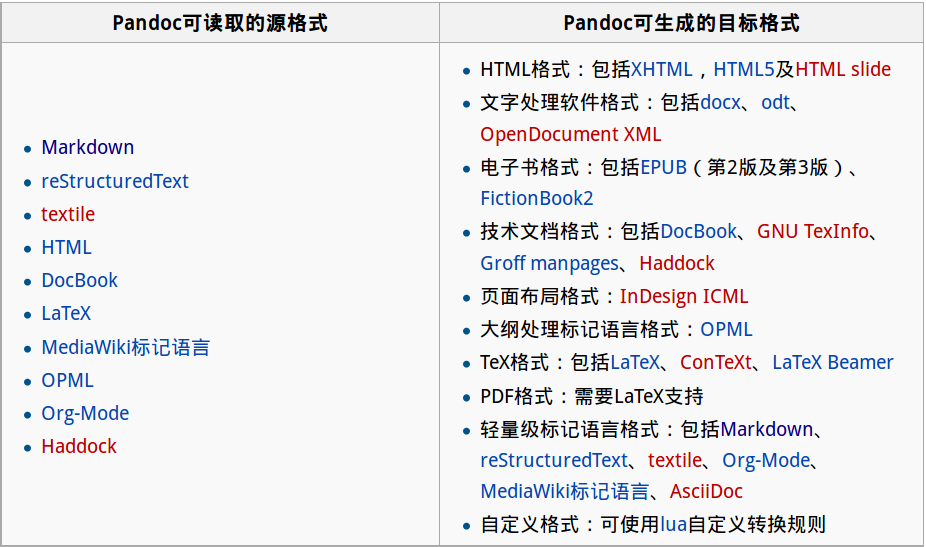
\includegraphics[width=12cm]{c1.markdown.pandoc.format.png}
  \end{figure}
\end{frame}

\begin{frame}[fragile]
  \frametitle{格式转换 | pandoc | 使用}
\begin{lstlisting}[language=bash]
# 安装
sudo apt install pandoc
#sudo apt-get install pandoc

# 使用帮助
man pandoc
pandoc -h

# 命令语法
pandoc [options] [input-file] ...
\end{lstlisting}
\end{frame}

\begin{frame}[fragile]
  \frametitle{格式转换 | pandoc | \alert{使用}}
\begin{lstlisting}[language=bash]
# Pandoc会根据文件的后缀名自动判断格式
pandoc -o output.html input.md

# 用户也可以显式地指定输入文件和输出文件格式
pandoc -f markdown -t html -o output.html input.md

# Markdown转HTML
pandoc input.md -o output.html -c Github.css
# Markdown转word
pandoc input.md -o output.docx -c Github.css
# Markdown转PDF(需要LaTeX)
pandoc input.md -o output.pdf --latex-engine=xelatex -V mainfont="SimSun" --template=template.latex
\end{lstlisting}
\end{frame}

\section{回顾与总结}
\subsection{总结}
\begin{frame}
  \frametitle{Markdown | 总结}
  \begin{block}{知识点}
    \begin{itemize}
      \item Markdown的基本语法:标题、引用、列表、代码、链接、强调……
      \item Markdown相关:knitr,pandoc
    \end{itemize}
  \end{block}
  \begin{block}{技能}
    \begin{itemize}
      \item 熟练使用Markdown撰写文档
      \item 能够使用pandoc转换文档格式
    \end{itemize}
  \end{block}
\end{frame}

\subsection{思考题}
\begin{frame}
  \frametitle{Markdown | 思考题}
  \begin{enumerate}
    \item 常见的文档样式(标题、强调等)如何使用Markdown语法来实现?
    \item 如何把Markdown文件转换成其他常见的文档格式?
  \end{enumerate}
\end{frame}

\begin{frame}
  \frametitle{下节预告}
  回顾shell编程的基础知识:
  \begin{itemize}
    \item 变量
    \item 操作符
    \item 条件流程控制
    \item 迭代流程控制
    \item 语法检查与调试
    \item ……
  \end{itemize}
\end{frame}


\section*{Acknowledgements}
\begin{frame}
  \frametitle{Powered by}
  \begin{center}
    
\includegraphics[width=9cm]{power.png}
  \end{center}
\end{frame}

\end{document}


